\section{Experimental Setup}
\label{sec:4}
% In this section, we discuss how to design the framework for discovering related articles in the corpus. As described in section \ref{sec:3}, each article contains semantic data including title, summary and content, together with meta-data, which consists of category, keywords, release date and the number of words/terms in the texts. The purpose of this section is to evaluate how the methods which are mentioned in section \ref{sec:2} work in effectiveness and efficiency together with different semantic data. Then the assessment of filtering method which reduces the number of candidates with combining the meta-data is analyzed. In other words, this section focuses on finding the answer of question 1 and 2.

The purpose of this section is to design experiments to evaluate how the STS methods which are aforementioned in section \ref{sec:2} work in effectiveness and efficiency together with different text fields. In addition, we also give the conditions, parameters and settings to support the experiments working. 

In section \ref{sec:4.1} the theoretical feasibility and challenge is discussed. The definition of terms and notations which are used in this section and the following sections is brought forwards in section \ref{sec:4.2}. In section \ref{sec:4.3} we discuss the architecture and the working procedure of the system. Section \ref{sec:4.4} mentions the design of experiments according to the application scenarios and depict the architecture of the framework. Furthermore, the setup of datasets which are used as training data and testing data is described in section \ref{sec:4.6} In the end, the list of the hardware and software which are applied for the experiments is enumerated in section \ref{sec:4.5} briefly.

\subsection{Theoretical Feasibility and Challenge}
\label{sec:4.1}

All methods which are introduced in section \ref{sec:2} are usually applied for computing the semantic similarity between documents. However, the objective of the system is to find related articles for given target articles. Foremost, the difference between the term \textit{similarity} and \textit{relatedness} must be understood. The terms \textit{similarity} and \textit{relatedness} are two separate concepts \cite{pedersen2007measures}. \textit{Similarity} is the measure which indicates how a text looks like another text semantically, while relatedness is a more general concept, which contain multiple notions, such as causal relationship, temporal relationship and the relationship shared the identical event or background. We illustrate the difference with two examples. More about errors will discuss in section \ref{sec:5.5}. 

\begin{description}
\item[Example 1] There are two pieces of news. One of them reports the football game of Euro Champions between FC Bayern and Real Madrid in 2014, while the other reports the football game of German Bundesliga between FC Bayern and Dortmund in 2015. Obviously, they are similar to each other semantically, because they share the same topic (football game) and the same subject (FC Bayern).Meanwhile, they are unrelated to each other. The reason is that the two games are held in the different seasons and the different competitions. Exactly, football games is quite a kind of short-term and event-sensitive events. In this example, we summarize that the documents are not similar in the most important topic leads to that they are unrelated to each other.
\item[Example 2] Consider two pieces of news, one reporting the terrorist attack in Europe and the other reporting Arab Spring. They are not similar, because both of topics and contents of the articles do not match to each other. However, they are related, because the second article is the background and partly origin of the first article. The judgement of relatedness requires pre-knowledge in this case. In this example, we consider that external knowledge is useful for obtaining text relatedness. 
\end{description}

From the two examples, we can draw a conclusion, that computing relatedness is much more complicated than computing similarity, because machines must understand exactly how human beings understand the identities and the differences between two articles as well as the significance degree thereof. However, \textit{similar} documents and \textit{related} documents have a non-negligible intersection normally. Our task is derived from a scenario of reality that two related articles need to be assigned for every target article. Therefore, it is unnecessary to find all possible related articles but it is acceptable to find only a subset of them. A way from computing \textit{similarity} to getting \textit{related} articles is feasible to attain the goal.

Certainly, discovery related articles using similarity methods leads to bias. It means, that the system prefers choosing articles only with specific characteristics as related articles and consequently some articles will never be assigned, e.g. articles which have the identical background with the target. The bias and error analysis are discussed in section \ref{sec:5.5}.

\subsection{Definition and Notions}
\label{sec:4.2}

In the following sections, a series of concepts are mentioned frequently. In order to avoid ambiguity and misapprehension, the definition and interpretation of these terms are given in the following list.

\begin{description}
\item[\texttt{Article}] an instance of a piece of news or report, which contains the complete information containing title, summary and content, which express in string form, and meta-data. Denoted as $D$.
\item[\texttt{Document}] a specific component of an article which refers to the string of content, title or summary. Without any explicit declaration, the document refers particularly to content. Denoted as $d$.
\item[\texttt{Candidate dataset}] the dataset in which all articles are as training data to build or update the model and used as candidates to be judged related articles. 
\item[\texttt{Candidate}] an instance in the candidate dataset.
\item[\texttt{Text field}] a general designation of title, summary and content of the article. 
\item[\texttt{N-gram field}] From each article $3\times3=9$ different outcomes are generated after preprocessing phase. They are unigram-content, bigram-content, trigram-content, unigram-title, bigram-title, trigram-title, unigram-summary, bigram-summary and trigram-summary. The general designation of the set of each kind of outcomes is called a n-gram field (abbr. NGF). 
\item[\texttt{Token}] the elementary semantic unit of a document.
\item[\texttt{Word}] (in the n-gram models) the elementary semantic unit of a document, which consists of $n$ adjacent tokens. ``Word'' is the same concept of ``token'', when $n$ equals $1$. In the case of $n > 1$, the concept ``phrase'' is more precise. However, we still use the uniform notion ``word'', to avoid the possible confusion. Denoted as $w_i$. 
\item[\texttt{Vocabulary}] the set of words which occur in the corpus. In VSMs, the vocabulary contains the words which occur in the corpus at least $k$ times (in our case, $k=5$), in order to reduce the dimension of term-weighted vectors. 
\item[\texttt{Term}] the unique item of the vocabulary $V$ which is generated by the entire corpus. Denoted as $t_i \in V$. 
\item[\texttt{Related-graph}] the graph in which the vertices are connected to each other according to the recommendation relationship which is stored in the corpus. If a path with two vertices exists, the corresponding articles are regarded as related to each other with the length $h$ of the path. Denoted the two articles are related with \textbf{$h$-hop}.

\label{tab:def_terms}
\end{description}


\subsection{Architecture of System and Experiments Design}
\label{sec:4.3}

The high-level architecture of the system was already depicted in figure \ref{fig:highlevel}. In this subsection, we explain how the system discovers related articles. 

The system consists of four components including preprocessing, model building, similarity computing and model updating. The architecture of the system is illustrated in figure \ref{fig:unsupervised}. 

\begin{figure}[!htb]
    \centering
    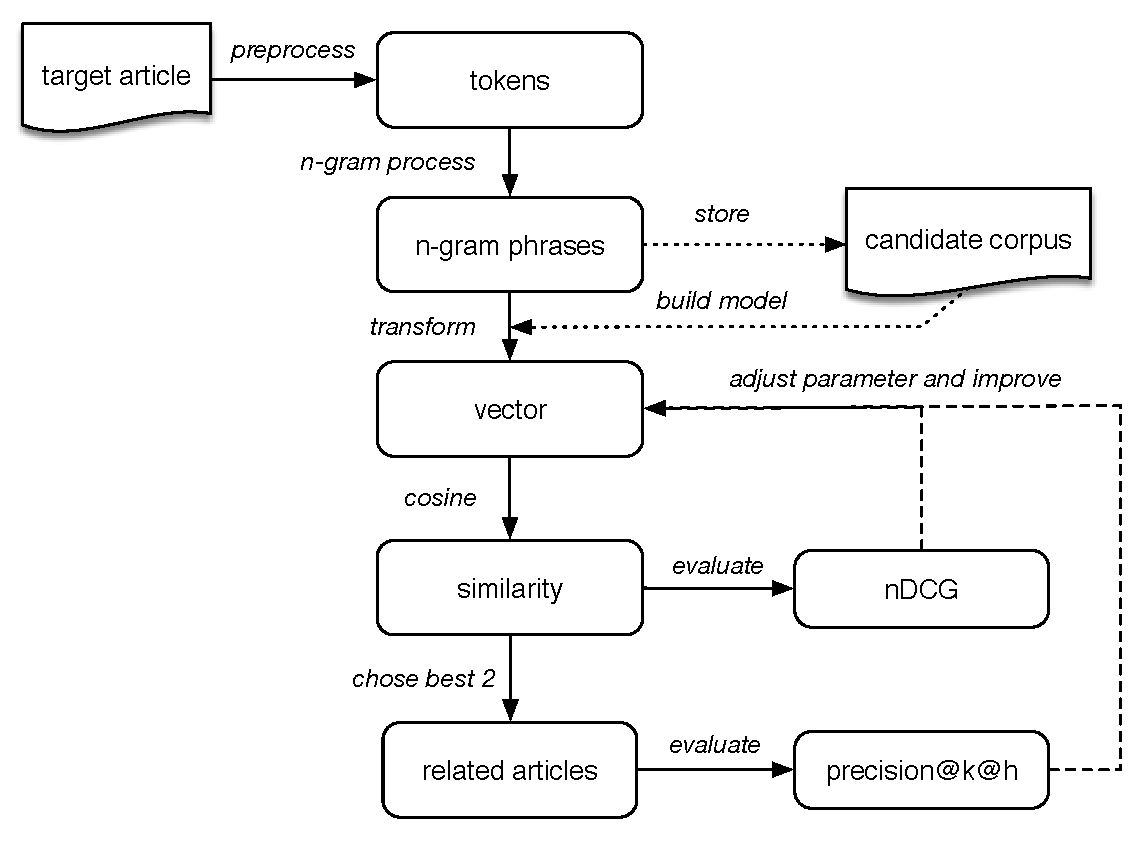
\includegraphics[width=0.7\textwidth]{fig/unsupervise}
    \caption{The architecture of the system to discover related articles.}
    \label{fig:unsupervised}
\end{figure}

\subsubsection{Preprocessing}
The original data of title, summary and content is stored in the strings in HTML format. After all markups are removed and all characters are converted to small case, a preprocessing method separates the strings into the respective sequences of tokens. Four alternative methods are explained as follows:

\begin{description}
\item[\texttt{\underline{SP}lit}] The string is splitted into a sequence of tokens by the special characters (whitespace, hyphen and punctuations). 
\item[\texttt{\underline{S}t\underline{E}m}] Tokens, which are the results from the method \textit{SP} are replaced by the respective stems. For example, ``book'' is the stem of ``books'', ``booking'' and ``booked''. The advantage of stemming is to reduce the vocabulary size and decrease computational complexity and avoid overfitting of building semantic models. However, stemming causes the problem of polysemy. 
\item[\texttt{\underline{ST}op}] After \textit{SP}, the stopwords, which are the most common words in a language, such as pronouns and prepositions, are filtered out from the sequence. 
\item[\texttt{\underline{S}tem+\underline{S}top}] The data is handled by both of \textit{SP} and \textit{SE}. 
\end{description}

\subsubsection{Model Building and Similarity Computing}

The component of model building is the crucial part exclusive for VSMs. The approaches of different STS methods are quite different. The detailed ways are described in the following list respectively.

\begin{description}
\item[\texttt{Jaccard}] Jaccard is distinct from VSMs, because there is no actual building phase. The so-called building phase is just to represent documents to sets of terms. The phase of similarity computing is that the term sets of the two articles are used for computing Jaccard coefficient.  
\item[\texttt{BoW}] BoW is the basic model in VSMs. Each document is represented as a vector, in which the weight of each dimension is the occurrence frequency of the corresponding term. The BoW vector of a given document is independent of the rest corpus, so long as the vocabulary is constant.
\item[\texttt{\tfidf{}}] \tfidf{} is the model based on BoW. Unlike BoW, the \tfidf{} vector is dependent on the document frequency and hence is sensitive to the change of the corpus. The applied tool to build \tfidf{} model is \textit{gensim}\footnote{gensim is a NLP tool, which focuses on topic modeling and retrieving semantically similar documents \cite{rehurek_lrec}. Official website: \url{https://radimrehurek.com/gensim/}}.
\item[\texttt{LSI} and \texttt{LDA}] We build model LSI and model LDA based on \tfidf{}. The function of models is to represent term-weighted vectors to topic-weighted vectors. In the both models, the hyperparameter is the number of topics, which impacts the quality of the semantic representation and the complexity of computation. It is therefore necessary to determine the optimal number of topics, in order to make balance between the quality and computational performance. 
\end{description}

In VSMs, each document is transformed as a vector and the semantic similarities to other documents are the \textit{cosine} similarities between the vector of the target document and the vectors of candidate documents. Two articles which have the greatest score in the candidate dataset to the given target article are predicted as the related articles. 
\subsubsection{Model Updating}

In the application scenario of reality, the candidate dataset is not constant but increases over time. Once an article is ready to publish, the system should select two articles with the greatest relatedness to the current article from the dataset. After the article released, it should be stored into the candidate dataset immediately and becomes a candidate of related articles to future articles. Therefore, the amount of the dataset will increase throughout. In the mean time, the characteristics of the dataset, for example, the topic distribution and the occurrence of new popular words, are rearranged over time. It is thereby necessary to update the model incrementally, in order to be capable of reflecting the recent state of the dataset in time. However, the computational time cost of model updating must be taken into account. Accordingly, one of the research tasks is to find the trade-off between the interval of updating and the impact on the performance of the effectiveness.  

\subsection{Experiment Description}
\label{sec:4.4}

The evaluation of the system is divided into two parts: static and dynamic evaluation. In the static evaluation, we focuses on the intrinsic performance including effectiveness and efficiency of the STS methods for the different NGF, when the candidate dataset and the target dataset are constant during the execution of the experiment. Accordingly, the objective of the first experiment is evaluate the performance of different STS methods in different NGF. Furthermore, how useful the different text fields and n-gram models are in relatedness computation and how different the STS methods perform in different NGF are analyzed. In the end, the system selects the method of best performance in each NGF. 

The dynamic evaluation concentrates on the availability of the models in the scenario of reality. To be specific, the second experiment is more interested in the fluctuate of performance, if the candidate dataset keeps increasing and the model needs updating incrementally. In addition, we attempt to find the balance between effectiveness and efficiency. The experiment sets up one evaluated system and two controlled system and evaluates them respectively. In brief, one controlled system refers to the theoretic lower bound of the system which has only old information and the other one refers to the theoretic upper bound of the system which maintains the complete information. The details of the controlled systems are described in section \ref{sec:5.4}. The performance characteristics of the evaluated system are discovered explicitly by comparing it with the controlled systems. 

\subsection{Dataset Setup}
\label{sec:4.6}

We setup the training and testing datasets from the ZEIT-corpus. Articles, which have no related articles or no \ititle{} field, or whose \icontent{} is less than 1000 characters, are filtered. Furthermore, articles which belong to a weak category \footnote{Weak category: the amount of articles in this category is fewer than $1\%$ of the corpus size} or which were released before 2009 are also removed from the corpus. Consequently, we have $75908$ articles in $7$ categories. The category distribution is drawn in table \ref{tab:cate_dist_new} and the release date distribution is in table \ref{tab:release_dist_new}. 

We separate the corpus into the (initial) training dataset and the testing dataset in different strategies for two experiments respectively. 

\begin{description}
\item[Experiment 1] $2000$ articles are selected randomly from the corpus as the testing dataset, and the rest articles are as the training data to train the models and as the candidates. 
\item[Experiment 2] The articles in corpus are sorted by the \textit{release date}, such that the real-world scenario can be simulated. The articles, which were published before 2013, are as the training data to initialize models. Meanwhile, the articles released after 2013 are as the testing dataset.

\end{description}

\begin{table}[!ht]
\centering
\begin{minipage}[b]{.48\linewidth}
\centering
\begin{tabular}{rrr}
\hline
\textbf{category} &   \textbf{quantity} &   \textbf{proportion (\%)} \\
\hline
Politik      &      26071 &            34.35 \\
Wirtschaft   &      12531 &            16.51 \\
Kultur       &       8584 &            11.31 \\
Gesellschaft &       7646 &            10.07 \\
Wissen       &       5273 &             6.95 \\
Sport        &       4993 &             6.58 \\
Digital      &       3887 &             5.12 \\
Reisen       &       2199 &             2.90 \\
Karriere     &       2169 &             2.86 \\
Studium      &       1570 &             2.07 \\
Lebensart    &        985 &             1.30 \\
\hline
\textbf{total}        &      75908 &           100.00 \\
\hline
\end{tabular}
\caption{Category distribution of \textit{ZEIT} corpus after filtering unsatisfied articles}
\label{tab:cate_dist_new}

\end{minipage}
\begin{minipage}[b]{.48\linewidth}
\centering
\begin{tabular}{rrr}
\hline
\textbf{year} &   \textbf{quantity} &   \textbf{proportion (\%)} \\
\hline
2009 & 12628 &            16.64 \\
2010 & 14716 &            19.39 \\
2011 & 13970 &            18.40 \\
2012 & 14583 &            19.21 \\
2013 & 14941 &            19.68 \\
2014 &  5070 &             6.68 \\
\hline
\textbf{total} & 75908 &           100.00 \\
\hline
\end{tabular}
\caption{Release date distribution of \textit{ZEIT} corpus after filtering unsatisfied articles}
\label{tab:release_dist_new}
\end{minipage}
\end{table}

\clearpage

\subsection{Hardware and Software}

The system is running on a Linux server. The detailed information of the server is drawn in table \ref{tab:pcinfo}.

\begin{table}[!htb]
%\centering
\begin{tabular}{ll}
CPU & Intel Xeon CPU E5420 @ 8 $\times$ 2.50GHz \\
RAM & 32GB \\ 
Disk & 3TB HDD \\ 
System & Debian GNU/Linux 7.7, 64 bits \\ 
Runtime & Python 3.4 \\
DBMS & MongoDB v3.2.5\\ 
Persistance & HDF5, gzip compressed \\
Externel Packages & NLTK, gensim, scikit-learn, pandas \\
\end{tabular}
\caption{General view of the hardware, system and software to be in use. }
\label{tab:pcinfo}
\end{table}
